\subsection{Captive}

\begin{frame}{The Captive Cross-Architectural Hypervisor}

\end{frame}

\begin{frame}{The Captive Cross-Architectural Hypervisor}

\centering
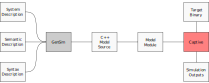
\includegraphics[width=\textwidth]{figures/gensim-toolflow-captive}

\end{frame}

\begin{frame}{The Captive Cross-Architectural Hypervisor}

Alternative full-system simulation tool which uses GenSim ADL models

\begin{itemize}
	\item Uses x86 virtualisation features
	\item Supports ARMv7 and ARMv8 (AArch64)
	\item Some host machine devices can also be used
\end{itemize}

\end{frame}

\begin{frame}{MMU Virtualisation}

In full-system simulation, one of the largest performance costs is virtual-physical address translations.

\begin{itemize}
	\item Need to check privileges
	\item Perform actual address translation
	\item Trigger exception if necessary
\end{itemize}

Most simulators speed up this process using a software cache

\end{frame}

\begin{frame}{MMU Virtualisation in Captive}

Captive avoids this cost by using the host MMU to perform translations:

\begin{itemize}
\item The host page table is set up to mimic the guest page table
\item Host privilege levels used to track guest privilege levels
\item Host memory faults can be used to model guest faults
\end{itemize}

\end{frame}

\begin{frame}
\centering
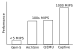
\includegraphics{figures/comparison-chart-captive}
\end{frame}

\begin{frame}{Captive - Host Virtualisation Features}

Many possible x86 features which could be used:

\begin{itemize}
	\item Intel-VT (or AMD-V)
	\item Memory Protection Keys
	\item Process Context IDs
	\item Privileged Execution
	\item Interrupts/Exceptions
	\item ...
\end{itemize}

\end{frame}
